\begin{spacing}{2}
    \section{实验}
\end{spacing}
\subsection{网络初始化设计}
使用Adam Optimizer,经过初步实验,学习率定为$1^{-5}$,并使用指数衰减学习率,衰减率设为0.95。卷积核使用Xavier初始化方法。实验共进行三组,具体参数如表\ref{Tab:test}所示。
\begin{table}[t]
    \centering
    \caption{损失函数}
    \label{Tab:test}
    \scalebox{1.0}{
        \begin{tabular}{ccc}
            \toprule  %添加表格头部粗线
            组别& 损失函数& 参数\\
            \midrule  %添加表格中横线
            第一组& 交叉熵& / \\
            第二组& 带权重交叉熵& 背景:1.2;房屋:0.8 \\
            第三组& 类别平衡交叉熵& / \\
            \hline \hline
        \end{tabular}
    }
    \vspace{10mm}
\end{table}
\subsection{实验结果}
经过1200次左右迭代,训练时间约12小时。由于每经过350次左右的迭代,系统会有一次不明原因的内存泄漏导致,因此下方的折线图只有350轮左右的迭代数据。
\subsubsection{第一组}
最初损失为3.5左右,最终损失降至0.35左右\ref{Fig:loss_1},正确率在0.85左右。
\begin{figure}[!t]
    \centering
    \includegraphics[width=1\textwidth]{Figures/group_1/loss.png}
    \caption{第一组损失}
    \label{Fig:loss_1}
\end{figure}
\begin{figure}[!t]
    \centering
    \includegraphics[width=1\textwidth]{Figures/group_1/accuracy.png}
    \caption{第一组正确率}
    \label{Fig:loss_1}
\end{figure}
\begin{figure}[!t]
    \centering
    \includegraphics[width=1\textwidth]{Figures/group_1/结果.png}
    \caption{第一组输出样例}
    \label{Fig:loss_1}
\end{figure}
\subsubsection{第二组}
最初损失为1.4左右,最终损失降至0.29左右\ref{Fig:loss_1},正确率在0.88左右,收敛速度较第一组快。
\begin{figure}[!t]
    \centering
    \includegraphics[width=1\textwidth]{Figures/group_2/loss.png}
    \caption{第二组损失}
    \label{Fig:loss_2}
\end{figure}
\begin{figure}[!t]
    \centering
    \includegraphics[width=1\textwidth]{Figures/group_2/accuracy.png}
    \caption{第二组正确率}
    \label{Fig:loss_2}
\end{figure}
\begin{figure}[!t]
    \centering
    \includegraphics[width=1\textwidth]{Figures/group_2/结果.png}
    \caption{第二组输出样例}
    \label{Fig:loss_2}
\end{figure}
\subsubsection{第三组}
最初损失为1.7左右,最终损失降至0.32左右\ref{Fig:loss_3},正确率在0.86左右,收敛速度介于第一组和第三组之间。
\begin{figure}[!t]
    \centering
    \includegraphics[width=1\textwidth]{Figures/group_3/loss.png}
    \caption{第三组损失}
    \label{Fig:loss_3}
\end{figure}
\begin{figure}[!t]
    \centering
    \includegraphics[width=1\textwidth]{Figures/group_3/accuracy.png}
    \caption{第三组正确率}
    \label{Fig:loss_3}
\end{figure}
\begin{figure}[!t]
    \centering
    \includegraphics[width=1\textwidth]{Figures/group_3/结果.png}
    \caption{第三组输出样例}
    \label{Fig:loss_3}
\end{figure}
\subsection{分析及改进}
以上都是较好的结果。但在这其中还是有许多问题的。以下是几个典型的问题。
\paragraph{建筑过大}
由于本次统一将图片裁成$256\times 256$大小,因此有些过大的建筑在整张图像中有所缺失。如\ref{Fig:big_building},本应整张图片都被识别为建筑,但是由于该建筑的范围超过了$256\times256$,因此未能完全识别。
\begin{figure}[!t]
    \centering
    \includegraphics[width=1\textwidth]{Figures/错误/建筑过大.png}
    \caption{建筑过大}
    \label{Fig:big_building}
\end{figure}
同样的错误还出现在中等大小的建筑上,如\ref{Fig:middle_building}。由于感受野大小不能包含整个建筑,所以建筑的中央未能正确识别为建筑。
\begin{figure}[!t]
    \centering
    \includegraphics[width=1\textwidth]{Figures/错误/中等建筑.png}
    \caption{中等大小建筑错误}
    \label{Fig:middle_building}
\end{figure}
\paragraph{错认}
另一类典型错误是将道路和汽车错认为房屋\ref{Fig:error_road}。由于道路和房屋的边缘比较相像,所以常有道路被错认为房屋的情况出现。
\begin{figure}[!t]
    \centering
    \includegraphics[width=1\textwidth]{Figures/错误/道路错认.png}
    \caption{道路错认}
    \label{Fig:error_road}
\end{figure}
另外,并排停放的汽车大小和形状与小型房屋相似,也经常被错认为房屋\ref{Fig:error_car}。
\begin{figure}[!t]
    \centering
    \includegraphics[width=1\textwidth]{Figures/错误/汽车错认.png}
    \caption{汽车错认}
    \label{Fig:error_car}
\end{figure}
\paragraph{树木和光影}
树木遮挡是造成误差的另外一个主要原因\ref{Fig:tree_error}。后期可能可以通过霍夫变换找到规则建筑的边界补齐。
\begin{figure}[!t]
    \centering
    \includegraphics[width=1\textwidth]{Figures/错误/树木遮挡.png}
    \caption{树木遮挡}
    \label{Fig:tree_error}
\end{figure}
另外由于该图像集中建筑屋顶都较周围物体明亮,因此一些屋顶过暗的建筑可能不能被正确识别\ref{Fig:dark_building}。
\begin{figure}[!t]
    \centering
    \includegraphics[width=1\textwidth]{Figures/错误/建筑过暗.png}
    \caption{建筑过暗}
    \label{Fig:dark_building}
\end{figure}
\subsection{最终结果}
最终选取了两张图片进行测试。一张建筑较为密集,一张建筑较为分散。原图尺寸为$5000\times 5000$,将其缩小到$4096\times 4096$。由于CPU性能限制,所以分别切成16张$1024\times1024$大小的图片进行运算后再拼接。得到的结果图又进行了开运算,结果如图所示。
